% Note technique : charge et décharge d'un condensateur
% Compilation : xelatex paper.tex   (deux fois)
% Les figures et numbers.tex sont produits par make_figures.py.
\documentclass[a4paper,11pt]{article}

\usepackage[margin=2.4cm]{geometry}
\usepackage{fontspec}
\usepackage{unicode-math}
\setmainfont{Latin Modern Roman}
\setsansfont{Latin Modern Sans}
\setmonofont{Latin Modern Mono}
\setmathfont{Latin Modern Math}
\usepackage{polyglossia}
\setmainlanguage{french}
\usepackage{amsmath}
\usepackage{booktabs}
\usepackage{graphicx}
\usepackage{caption}
\usepackage{microtype}
\usepackage[european]{circuitikz}
\usepackage[hidelinks]{hyperref}
% Généré par make_figures.py à partir de data/results.json — ne pas modifier à la main.
\newcommand{\slopeEE}{\ensuremath{1{,}01}}
\newcommand{\slopeBE}{\ensuremath{0{,}99}}
\newcommand{\slopeTR}{\ensuremath{2{,}00}}
\newcommand{\errEE}{\ensuremath{11{,}8}}
\newcommand{\errBE}{\ensuremath{7{,}7}}
\newcommand{\errTR}{\ensuremath{0{,}79}}
\newcommand{\vLastTwoFive}{\ensuremath{4{,}4}}
\newcommand{\RIdeal}{\ensuremath{4{,}55}}
\newcommand{\tRreal}{\ensuremath{1{,}033}}
\newcommand{\tRerr}{\ensuremath{3{,}3}}
\newcommand{\tolLow}{\ensuremath{-10{,}9}}
\newcommand{\tolHigh}{\ensuremath{11{,}1}}
\newcommand{\tolStd}{\ensuremath{5{,}8}}
\newcommand{\ripple}{\ensuremath{0{,}62}}
\newcommand{\energyJ}{\ensuremath{12{,}5}}


\newcommand{\dd}{\mathrm{d}}
\newcommand{\ee}{\mathrm{e}}
\captionsetup{font=small,labelfont=bf}
\setlength{\parindent}{0pt}
\setlength{\parskip}{0.55em}

\title{Charge et décharge d'un condensateur :\\ modèle RC et comparaison de schémas d'intégration}
\author{Thomas}
\date{octobre 2026}

\begin{document}
\maketitle

\begin{abstract}
\noindent On établit la réponse d'un condensateur à un échelon de tension à travers une résistance, puis on la compare à trois schémas d'intégration numérique de pas constant (Euler explicite, Euler implicite, trapèzes). Les ordres de convergence mesurés sont \slopeEE, \slopeBE{} et \slopeTR, et la condition de stabilité $h<2\tau$ du schéma explicite est vérifiée. L'énergie dissipée dans la résistance vaut $\tfrac12 CV^2$ quelle que soit $R$. Ce travail est théorique et numérique : aucune mesure sur banc n'a encore été faite.
\end{abstract}

\section{Modèle}
Une source $v_s$ charge un condensateur $C$ à travers une résistance $R$ (figure~\ref{fig:circuit}). La loi des mailles et la relation $i=C\,\dd v_C/\dd t$ donnent
\begin{equation}\label{eq:ode}
  \tau\,\frac{\dd v_C}{\dd t}+v_C=v_s(t),\qquad \tau=RC .
\end{equation}
Pour $v_s=V$ constante et $v_C(0)=v_0$ :
\begin{equation}\label{eq:sol}
  v_C(t)=V+(v_0-V)\,\ee^{-t/\tau},\qquad i(t)=\frac{V-v_0}{R}\,\ee^{-t/\tau}.
\end{equation}
Le temps de montée 10--90\,\% vaut $t_r=\tau\ln 9\approx 2{,}197\,\tau$ ; avec la fréquence de coupure $f_c=1/(2\pi\tau)$, on obtient $t_r f_c=\ln 9/(2\pi)\approx 0{,}350$.

\begin{figure}[h]
  \centering
  \begin{circuitikz}[scale=0.95, transform shape]
    \draw (0,0) to[V=$v_s$] (0,2.4) to[R=$R$, i=$i$] (4,2.4) to[C=$C$, v=$v_C$] (4,0) -- (0,0);
    \draw (2,0) node[ground]{};
  \end{circuitikz}
  \caption{Circuit RC série.}\label{fig:circuit}
\end{figure}

\section{Intégration numérique}
On résout \eqref{eq:ode} avec $x=h/\tau$ et $v_{k+1}=a\,v_k+b$ (tableau~\ref{tab:schemas}). Le facteur d'amplification $a$ gouverne la stabilité : pour Euler explicite, $\lvert 1-x\rvert<1$ impose $h<2\tau$. Avec $h=\tau/2$ (figure~\ref{fig:transient}), l'erreur maximale rapportée à $V$ est de \errEE\,\% (Euler explicite), \errBE\,\% (Euler implicite) et \errTR\,\% (trapèzes). Avec $h=2{,}5\,\tau$, la solution explicite diverge : après trois pas, $v=\vLastTwoFive\,V$.

\begin{table}[h]
  \centering
  \caption{Schémas d'intégration pour $\tau\,\dot v=V-v$ ; $x=h/\tau$.}\label{tab:schemas}
  \begin{tabular}{llcl}
    \toprule
    Schéma & Facteur d'amplification $a$ & Ordre & Stabilité \\
    \midrule
    Euler explicite & $1-x$ & 1 & $h<2\tau$ \\
    Euler implicite & $1/(1+x)$ & 1 & inconditionnelle \\
    Trapèzes & $(1-x/2)/(1+x/2)$ & 2 & inconditionnelle \\
    \bottomrule
  \end{tabular}
\end{table}

\begin{figure}[h]
  \centering
  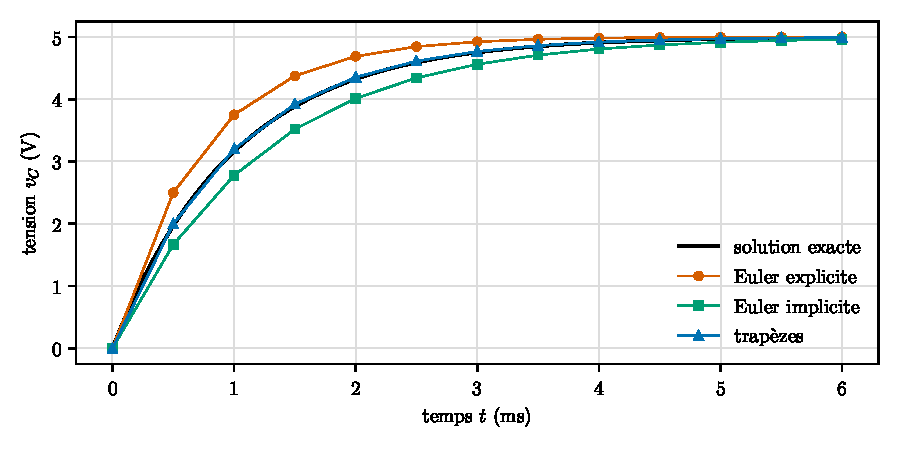
\includegraphics[width=0.92\linewidth]{fig-transient.pdf}
  \caption{Charge de $C=1\ \mu$F à travers $R=1$ k$\Omega$ sous $V=5$ V ($\tau=1$ ms), pas $h=\tau/2$.}\label{fig:transient}
\end{figure}

En faisant varier $h$ de $\tau$ à $\tau/256$ environ, les pentes mesurées en échelle logarithmique (figure~\ref{fig:conv}) sont \slopeEE, \slopeBE{} et \slopeTR{} : les schémas sont d'ordre 1, 1 et 2, comme attendu.

\begin{figure}[h]
  \centering
  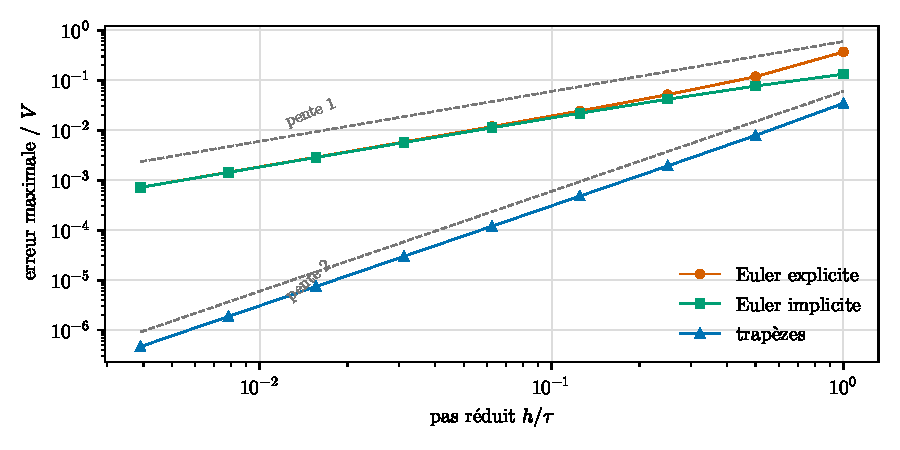
\includegraphics[width=0.92\linewidth]{fig-convergence.pdf}
  \caption{Erreur maximale sur $[0,6\tau]$ en fonction du pas.}\label{fig:conv}
\end{figure}

\section{Énergie et dimensionnement}
L'énergie dissipée dans $R$ pendant la charge depuis zéro est
\begin{equation}\label{eq:energy}
  E_R=\int_0^\infty R\,i^2\,\dd t=\frac{V^2}{R}\cdot\frac{\tau}{2}=\tfrac12 CV^2 ,
\end{equation}
indépendante de $R$ ; l'intégration numérique donne \energyJ\ $\mu$J pour $C=1\ \mu$F et $V=5$ V, pour $R=100\ \Omega$, $1$ k$\Omega$ et $10$ k$\Omega$. Le rendement d'une charge résistive est donc de 50\,\%.

Pour $t_r=1$ ms avec $C=100$ nF, il faut $R=\RIdeal$ k$\Omega$ ; la valeur E12 la plus proche, $4{,}7$ k$\Omega$, donne $t_r=\tRreal$ ms (écart de $+\tRerr\,\%$). Avec $R$ à $\pm1\,\%$ et $C$ à $\pm10\,\%$, $\tau$ varie au pire de \tolLow\,\% à $+\tolHigh\,\%$ ; l'écart type est de \tolStd\,\% pour des lois uniformes indépendantes.

\section{Limites et perspectives}
Le modèle ignore la résistance série équivalente, l'inductance parasite, les fuites et la variation de la capacité effective sous tension continue. Une validation sur banc (générateur 0--5 V, oscilloscope) reste à faire ; elle permettra de confronter $\tau$ et $t_r$ mesurés aux prévisions.

\begin{thebibliography}{9}
\bibitem{hh} P. Horowitz, W. Hill, \emph{The Art of Electronics}, 3\textsuperscript{e} éd., Cambridge University Press, 2015.
\bibitem{hw} E. Hairer, G. Wanner, \emph{Solving Ordinary Differential Equations II : Stiff and Differential-Algebraic Problems}, 2\textsuperscript{e} éd., Springer, 1996.
\bibitem{nagel} L. W. Nagel, \emph{SPICE2 : A Computer Program to Simulate Semiconductor Circuits}, mémo ERL-M520, University of California, Berkeley, 1975.
\end{thebibliography}

\end{document}
